%!TEX root = Main.tex

\section{The first Section}

  Content in first section \cite{Chin_DMR_ICCAD2013}

   

\section{Flow of Our Framework}
  \begin{figure}[ht]
    \centering
    \centerline{
      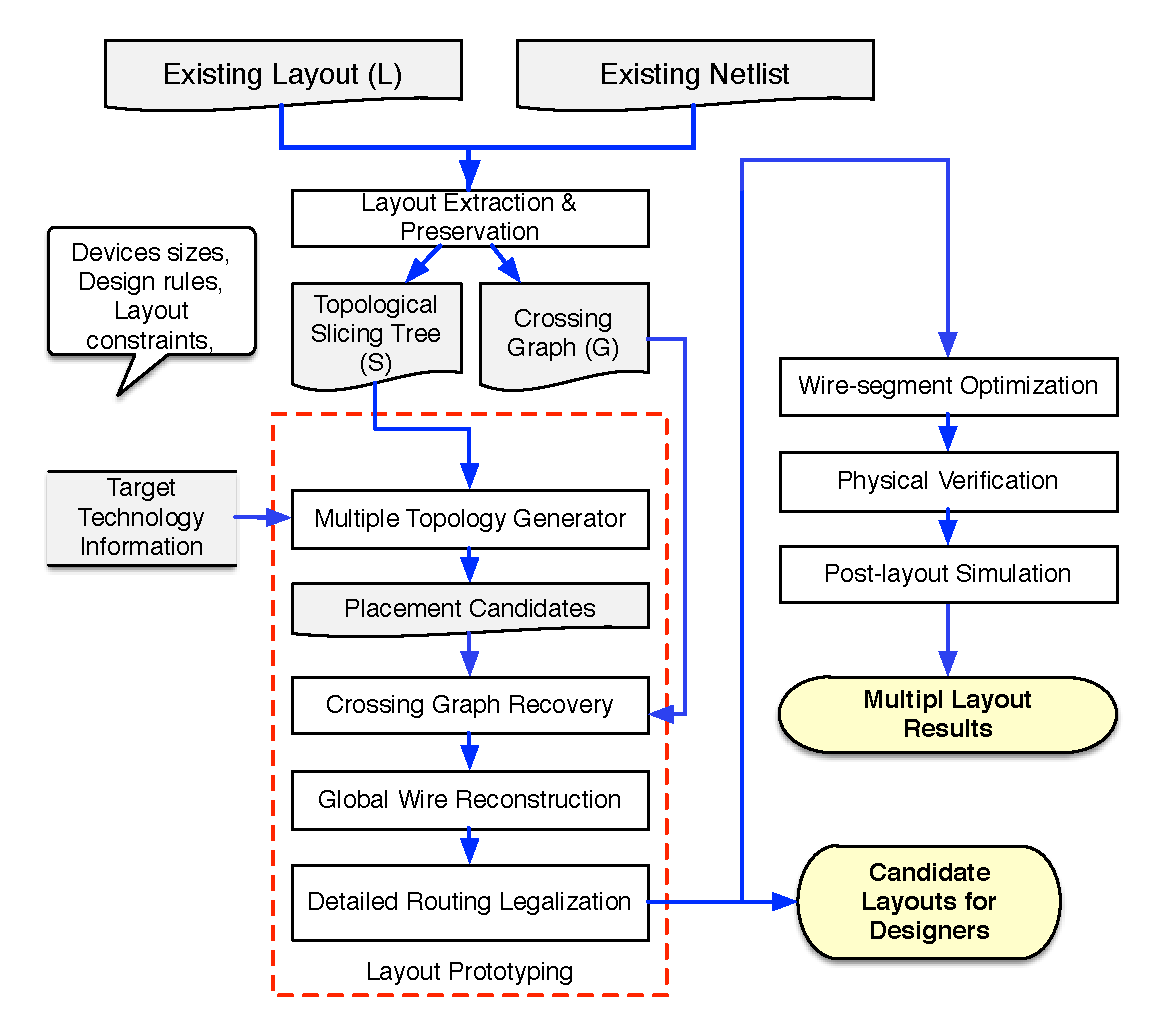
\includegraphics[width=0.5\textwidth]{Fig/proto_flow.eps}
    }
    \caption{Overall flow of the proposed layout migration framework.} 
    \label{fig:Flow}
  \end{figure}


  In order to provide fast prototyping for layout migration, this software extracted the reference layout with placement and routing respectively. The migrated layout is generated according to the extracted information. and then it dumps into real design after physical verification for performance simulation. Fig.~\ref{fig:Flow} shows the overall flow diagram of our methodology.
  The flow is mainly separated into three stages: 
  \begin{enumerate}
    \item {\bf Extraction and Preservation}: A layout extraction and preservation technique \cite{Chin_DMR_ICCAD2013} can not only be applied to generalized layout, but also hierarchical design.
    \item {\bf Prototyping}: The preserved topology of original layout can be generated into multiple layout candidates with placement and routing. 
    \item {\bf Wire optimization}: A detailed routing refinement is applied automatically to route the unrouted nets for final verification and simulation.
  \end{enumerate}

  In the end, a set of layouts with refinement is obtained, which provides designers a quick look of possible solutions that can be used. The layout results are automatically dumped into industrial layouts for demonstration and simulation. 


\section{Program Setting and Results}
  
  Our Software is developed with g++ 4.1.2 for methodology, Synopsys $\text{PyCell Studio}^{\text{TM} }$ 4.7.1 for layout realization and Qt 4.8.4 for GUI demonstration. We also display the layout with the reference one and the generated layout via $\text{Cadence}^{\text{\textregistered}}$ $\text{Virtuoso}^{\text{\textregistered}}$ 6.1.5. The migration of a variable-gain amplifier (VGA), a folded-cascode operational amplifier (OpAmp) and low dropout regulator (LDO) will be demonstrated step-by-step as applications to show the feasibility of our Software. 
  \begin{table}[ht]
      \begin{center}
      \scriptsize
      \caption{Specification of experimental circuits: OpAmp and VGA}\label{table:Spec}
      \begin{tabular}{|l|c|c|}
      \hline
        Circuit   & OpAmp & VGA \\ 
        \hline
        technology  & umc90nm & umc90nm     \\
        \hline
        $V_{dd}ㄌ$     & 1V    & 1.1V        \\
        \hline
        Load Capacitance  & 200pF & 1.5pF   \\
        \hline
        Gain    & $\geq 48.653dB$ & $\geq 18.48dB$      \\
        \hline
        Gain Bandwidth &  $\geq 100 MHz$ & $\geq 5MHz$      \\
        \hline
        Phase Margin  & $\geq 45deg$ & $\geq 45deg$     \\
        \hline
        Area    & 832.66 $\mu m^2$  & 10889.88 $\mu m^2$  \\
      \hline
      \end{tabular}
    \end{center}
  \end{table}
